\documentclass[aps,prd,amsfonts,amssymb,amsmath,nofootinbib,reprint,showpacs]{revtex4-1}
\usepackage{graphicx,color,psfrag}
\usepackage{mathrsfs}
\usepackage{dcolumn}
\usepackage{hyperref}

\newcommand{\eqnref}[1]{(\ref{eq:#1})}
\newcommand{\figref}[1]{Fig.\ \ref{fig:#1}}
\newcommand{\Figref}[1]{Fig.\ \ref{fig:#1}}
\newcommand{\secref}[1]{Sec.\ \ref{sec:#1}}
\newcommand{\Tabref}[1]{Table \ref{tab:#1}}

\newcommand{\units}[1]{\ensuremath{~\mathrm{#1}}}

\newcommand{\sub}[1]{\ensuremath{_\text{#1}}}
\newcommand{\super}[1]{\ensuremath{^\text{#1}}}
\newcommand{\dd}{\ensuremath{\text{d}}}
\newcommand{\diff}[2]{\ensuremath{\frac{\dd {#1}}{\dd {#2}}}}
\newcommand{\difftwo}[2]{\ensuremath{\frac{\dd^2 {#1}}{\dd {#2}^2}}}
\newcommand{\partialdiff}[2]{\ensuremath{\frac{\partial {#1}}{\partial {#2}}}}
\newcommand{\intd}[4]{\ensuremath{\int_{#1}^{#2}{#3}\,\dd{#4}}}
\newcommand{\recip}[1]{\ensuremath{\frac{1}{#1}}}
\newcommand{\grad}{\ensuremath{\boldsymbol{\nabla}}}
\newcommand{\order}[1]{\ensuremath{\mathcal{O}({#1})}}

\begin{document}

%\preprint{}

\title{Characterization of transient resonances in extreme-mass-ratio-inspirals}

\author{Robert H. Cole}
\email[]{rhc2@ast.cam.ac.uk}
\author{Christopher P.L. Berry}
\email[]{cplb2@ast.cam.ac.uk}
\author{Priscilla Ca\~{n}izares}
\email[]{pcm@ast.cam.ac.uk}
\author{Jonathan R. Gair}
\email[]{jgair@ast.cam.ac.uk}
\affiliation{Institute of Astronomy, Madingley Road, Cambridge, CB3 0HA, United Kingdom}

\date{\today}

\begin{abstract}
\end{abstract}

% 04.25.Nx 	Post-Newtonian approximation; perturbation theory; related approximations
% 04.30.-w 	Gravitational waves
% 04.70.-s 	Physics of black holes
% 98.62.Js 	Galactic nuclei (including black holes), circumnuclear matter, and bulges 
\pacs{04.25.Nx, 04.30.--w, 04.70.--s, 98.62.Js}

\maketitle

\section{Introduction}

In the prologue to his classic monograph, Chandrasekhar~\cite{Chandrasekhar1992} celebrates the simplicity of black holes (BHs). The Kerr solution is defined by just two parameters: mass and spin. Despite the baldness of the BH metrics, great intricacies manifest in their properties. This is made evident when a second body is introduced. The two-body problem in general relativity (GR) is well studied. It is of paramount importance for gravitational wave (GW) astronomy, where binary systems are the dominant source of radiation. Correctly modelling the dynamics of these systems is necessary to interpret and extract information from gravitational waveforms.

We have made progress in understanding the general relativistic two-body problem in recent years. Bodies of comparable mass can be studied using numerical relativity. Rapid advances in this field have been made following breakthroughs in 2005~\cite{Pretorius2005,Campanelli2006,Baker2006}. These simulations shall allow us to understand BH--BH mergers. Stellar-mass BH mergers are targets for ground-based GW detectors, such as the currently mid-upgrade LIGO~\cite{Harry2010} and Virgo~\cite{Accadia2011}, and the in-construction Kagra~\cite{Kuroda2010}. Massive BH mergers, expected to be the result of galaxy mergers, are potential sources for a space-borne detector such as eLISA~\cite{Amaro-Seoane2012a}. Systems of unequal masses are more challenging to evolve numerically as they complete a larger number of orbits and it is necessary to resolve two different scales. Calculations can instead be performed perturbatively. The paradigm unequal mass system has a stellar-mass BH orbiting a massive black hole. These extreme-mass-ratio inspirals produce GWs that are a promising signal for space-borne detectors~\cite{Amaro-Seoane2007}. Despite being well-studied there still remain open questions.

In the case of extreme-mass-ratio systems, efforts are concentrated on understanding the gravitational self-force~\cite{Barack2009,Poisson2004}. In the test particle limit the smaller body follows an exact geodesic of the BH's spacetime. Including the effects of the smaller body's finite mass, the background spacetime is perturbed. This back-reaction from this deformation alters the small body's orbital trajectory, and can be modelled as a self-force that moves the body from its geodesic. The self-force is commonly divided into two pieces, dissipative and conservative. The former encapsulates the slow decay of the orbital energy and angular momentum, constants of the motion in the test particle limit, through radiation. The latter shifts the orbital phases inducing precession.
%The dissipative piece is time-asymmetric and has the larger effect on the evolution of the orbital phase; the conservative piece is time-symmetric and has a smaller influence on the on the phase although this can accumulate over many orbits. % Check time-symmetry argument
Being able to accurately model the influence of the self-force shall allow us to create accurate waveform models.

Flanagan and Hinderer~\cite{Flanagan2012} highlighted a qualitatively new phenomenon that occurs in the general relativistic two-body problem, that of transient resonances. Geodesic orbits in GR have three associated frequencies: the radial frequency $\Omega_r$, the polar frequency $\Omega_\theta$ and the azimuthal frequency $\Omega_\phi$. The first two describe libration and the third rotation (except in the case of polar orbits where $\Omega_\theta$ also describes rotation)~\cite{Goldstein2002}. % Section 10.6
In the weak-field limit these all tend towards the Keplerian frequency; in the strong-field $\Omega_r < \Omega_\theta < \Omega_\phi$ and they may differ significantly. For extreme-mass-ratio systems, the evolution time-scale is much longer than the orbital period such that the motion of the smaller body is approximately geodesic over orbital time-scales. The evolution of the orbit can be approximated as a series of geodesics using the osculating element formalism~\cite{Pound2008,Gair2011a}. During this evolution the frequencies may become commensurate. Resonances occur when the radial and polar frequencies are rational multiples of each other:
\begin{equation}
\nu = \frac{\Omega_r}{\Omega_\theta} = \frac{n_\theta}{n_r},
\end{equation}
where $n_r$ and $n_\theta$ are integers (with no common factors). The azimuthal motion is not important because of the axisymmetry of the background spacetime. During resonance, terms in the self-force that usually average to zero can combine coherently, significantly impacting the motion~\cite{Flanagan2012a}.

Geodesic motion in Kerr spacetime can be described by use of the action--angle formalism~\cite{Goldstein2002}. % Chapter 10
We shall consider a body of mass $\mu$ orbiting a BH of mass $M$, where $\eta = \mu/M \ll 1$, and describe the motion in the directions of the standard Boyer--Lindquist coordinates using generalised angle variables $q_\alpha = \{q_t,q_r,q_\theta,q_\phi\}$ \citep{Hinderer2008}. We denote the integrals of the geodesic motion, the generalised action variables, by $J_A$. These are the energy per unit mass $E$, the axial angular momentum per unit mass $L_z$ and the Carter constant per unit mass squared $Q$~\cite{Carter1968}. The system evolves following~\cite{Flanagan2012}
\begin{subequations}
\begin{eqnarray}
\diff{q_\alpha}{\lambda} & = & \omega_\alpha(\boldsymbol{J}) + \eta g_\alpha^{(1)}(q_r,q_\theta,\boldsymbol{J}) + \order{\eta^2}; \\
\diff{J_A}{\lambda} & = & \eta G_A^{(1)}(q_r,q_\theta,\boldsymbol{J}) + \order{\eta^2},
\end{eqnarray}
\end{subequations}
where $\lambda$ is Mino time~\cite{Mino2003}, and the forcing functions $g_\alpha^{(1)}$ and $G_A^{(1)}$ originate from the first-order self-force. At zeroth order in the mass ratio we recover the limit of purely geodesic motion: the integrals of the motion are actually constants and the angle variables evolve according to their associated frequencies $\omega_\alpha$.

The leading order dissipative correction to geodesic motion is calculated following the adiabatic prescription~\cite{Hinderer2008}: by dropping the forcing term $g_\alpha^{(1)}$ (and all higher order terms) and replacing the the forcing term $G_A^{(1)}$ with its average over the $2$-torus parametrized by $q_r$ and $q_\theta$ $\langle G_A^{(1)}\rangle_{q_r,\,q_\theta}$~\cite{Drasco2005}. For most orbits this is sufficient, $G_A^{(1)}$ is given by its average value plus a rapidly oscillating component~\cite{Arnold1988}. % Chapter 5, section 1
However, this averaging fails when the ratio of frequencies is the ratio of integers. In this case the trajectory does not ergodically fill the $2$-torus but instead traces out a $1$-dimensional subspace.\footnote{For illustrations, see Grossman, Levin and Perez-Giz~\cite{Grossman2012}.} There are then contributions to the self-force that no longer average out beyond $\langle G_A^{(1)}\rangle_{q_r,\,q_\theta}$. Intuitively, we expect that this effect is more important for ratios of small integers as when the integers are large, the orbit comes close to all points on the $2$-torus.

In this work we seek to characterise the importance of these resonances for the purposes of modelling extreme-mass-ratio inspirals. This requires calculating the impact that passing through a resonance has on the orbital evolution and discovering for which resonances this is significant.

We use geometric units with $G = c = 1$ throughout. We always use $M$ for the mass of the central massive BH and $a$ as the spin parameter. We also use the dimensionless spin $a_\ast \equiv a/M$; we take the convention that $0 \leq a_\ast < 1$.

\section{Problem formulation}

\subsection{Kerr geodesics}

The evolution of an extreme-mass-ratio ($\eta \ll 1$) system is slow. Instantaneously, the motion of the orbiting mass can be described as geodesic, with the integrals of the motion changing on time-scales of many orbital periods. We analyse the behaviour of resonances with the osculating element framework, where the trajectory is described by a sequence of geodesics which each match onto the motion at a particular instance. It is therefore necessary to develop an understanding of the Kerr geodesics.

The geodesic equations may be written as~\cite{Carter1968, Chandrasekhar1992} % section 62
\begin{subequations}
\begin{eqnarray}
\diff{t}{\lambda} & = & a\left(L_z - aE\sin^2 \theta\right) + \frac{r^2 + a^2}{\Delta}\mathcal{T},\\
\diff{r}{\lambda} & = & \pm \sqrt{V_r},\\
\diff{\theta}{\lambda} & = & \pm \sqrt{V_\theta},\\
\diff{\phi}{\lambda} &  = & \frac{L_z}{\sin^2 \theta} - aE + \frac{a}{\Delta}\mathcal{T},
\end{eqnarray}
\end{subequations}
where $\Delta = r^2 - 2M r + a^2$; the signs of the $r$ and $\theta$ equations can be chosen independently, and we have introduced potentials
\begin{subequations}
\begin{eqnarray}
\mathcal{T} & = & E\left(r^2 +a^2\right) - aL_z,\\
V_r & = & \mathcal{T}^2 - \Delta\left[r^2 + \left(L_z -aE\right)^2 + Q\right],\\
V_\theta & = & Q - \cos^2 \theta\left[a^2\left(1 - E^2\right) + {\displaystyle \frac{L_z^2}{\sin^2\theta}}\right].
\end{eqnarray}
\end{subequations}
As an affine parameter we have used Mino time which is related to the proper time $\tau$ by~\cite{Mino2003}
\begin{equation}
\tau = \intd{}{}{r^2 + a^2 \cos^2\theta}{\lambda}.
\end{equation}
Using Mino time allows us to decouple the $r$ and $\theta$ motions.

We only consider bound motion~\cite{Wilkins1972}. The radial motion covers a range $r\sub{p} \leq r \leq r\sub{a}$ where the turning points are the periapsis $r\sub{p}$ and apoapsis $r\sub{a}$. Drawing upon Keplerian orbits we parametrize the motion using
\begin{equation}
r = \frac{p M}{1+e\cos\psi},
\end{equation}
introducing eccentricity $e$, (dimensionless) semilatus rectum $p$ and relativistic anomaly $\psi$~\cite{Darwin1961,Drasco2004}. Whilst $r$ oscillates between its maximum and minimum values, $\psi$ increases secularly increasing by $2\pi$ across an orbit. The poloidal motion covers a range $\theta_- \leq \theta \leq \pi - \theta_-$. We also parametrize this motion in terms of an angular phase $\chi$, according to~\cite{Hughes2000}
\begin{equation}
\cos\theta = \cos\theta_-\cos\chi.
\end{equation}
Whilst $\psi$ and $\chi$ are $2\pi$ periodic they are not the canonical action-angle variables~\cite{Schmidt2002}; they are, however, easy to work with.

The geodesic motion can equally be described by $\{E,L_z,Q\}$ or $\{p,e,\theta_-\}$~\cite{Schmidt2002}. Converting between them requires finding the solutions of $V_r = 0$ and $V_\theta = 0$. We employ a slightly different parameter set of $\{p,e,\iota\}$ where we have introduced the inclination~\cite{Ryan1996,Glampedakis2002}
\begin{equation}
\tan \iota = \frac{\sqrt{Q}}{L_z}.
\end{equation}
This is $0 \leq \iota < \pi/2$ for prograde orbits and $\pi/2 < \iota \leq \pi$ for retrograde orbits. Equatorial orbits ($\theta_- = \pi/2$) have $\iota = 0$ or $\pi$ and polar orbits ($\theta_- = 0$) have $\iota = \pi/2$. Whilst formulae exist for conversion between the different parameters, these are complicated and uninsightful, so we do not reproduce them here.\footnote{In practice we find turning points numerically.}

\subsection{Orbital resonances}

The radial and polar orbital periods in Mino time are given by
\begin{subequations}
\begin{eqnarray}
\Lambda_r & = & 2\intd{r\sub{p}}{r\sub{a}}{\recip{\sqrt{V_r}}}{r} = \intd{-\pi}{\pi}{\diff{\lambda}{\psi}}{\psi}, \\
\Lambda_\theta & = & 4\intd{\theta_-}{\pi/2}{\recip{\sqrt{V_\theta}}}{\theta} = \intd{-\pi}{\pi}{\diff{\lambda}{\chi}}{\chi}.
\end{eqnarray}
\end{subequations}
The orbital frequencies are thus
\begin{equation}
\Upsilon_r = \frac{2\pi}{\Lambda_r}, \quad \Upsilon_\theta = \frac{2\pi}{\Lambda_\theta}.
\end{equation}
The geodesic equations for coordinate time $t$ and azimuthal angle $\phi$ are just functions of $r$ and $\theta$, hence their evolutions can be expressed as Fourier series~\cite{Drasco2005}
\begin{subequations}
\begin{eqnarray}
\diff{t}{\lambda} & = & \sum_{k_r,\,k_\theta}T_{k_r,\, k_\theta}\exp\left[-i\left(k_r\Upsilon_r + k_\theta\Upsilon_\theta\right)\right], \\
\diff{\phi}{\lambda} & = & \sum_{k_r,\,k_\theta}\Phi_{k_r,\, k_\theta}\exp\left[-i\left(k_r\Upsilon_r + k_\theta\Upsilon_\theta\right)\right].
\label{eq:Mino-Fourier}
\end{eqnarray}
\end{subequations}
The $(0,\,0)$ coefficients in these series give the average secular rate of increase of these quantities. We define
\begin{equation}
\Gamma = T_{0,\,0}, \quad \Upsilon_\phi = \Phi_{0,\,0}
\end{equation}
to act as Mino time frequencies. We can now convert to coordinate time frequencies using
\begin{equation}
\Omega_r = \frac{\Upsilon_r}{\Gamma}, \quad \Omega_\theta = \frac{\Upsilon_\theta}{\Gamma}, \quad \Omega_\phi = \frac{\Upsilon_\phi}{\Gamma}.
\end{equation}

Transient resonances occur when the radial and poloidal motions are commensurate, when
\begin{equation}
\nu = \frac{\Upsilon_r}{\Upsilon_\theta} = \frac{\Omega_r}{\Omega_\theta} = \frac{n_\theta}{n_r}
\end{equation}
is the ratio of small integers. At this point any Fourier series like those in \eqnref{Mino-Fourier} goes from being an expansion in two frequencies to being an expansion in a single frequency~\cite{Bosley1992}.

On resonance, the radial and poloidal motions are locked together such that we could express one as a function of the other. For a general non-resonant orbit there is no fixed correlation between two coordinates. After a sufficiently long time, the trajectory comes arbitrarily close to every point in the range of motion (with $r\sub{p} \leq r \leq r\sub{a}$ and $\theta_- \leq \theta \leq \pi - \theta_-$); on account of the orbital precession, the whole space is densely covered. This does not happen on resonance as the trajectory keeps cycling over the same path. The points visited are controlled by the relative phases of the $r$ and $\theta$ motions. To represent this, we use the $r$ phase at the $\theta$ turning point $\psi_{\theta_-} = \psi(\chi = 0)$. Varying $\psi_{\theta_-}$ across its full range allows every point in the range of motion to be reached. Hence averaging over all values of $\psi_{\theta_-}$ for a resonant orbit is equivalent to averaging over the $\psi$--$\chi$ $2$-torus for non-resonant orbits.

One might be concerned about the nature of resonances following the inclusion of the self-force: true geodesic motion only exists at zeroth order in $\eta$ and, whilst it is a good approximation over short time-scales, for small $\eta$ there is a small disparity. The conservative piece of the self-force induces extra precession which leads to a slight shift in the orbital frequencies~\cite{Warburton2012}.\footnote{The Kolmogorov--Arnold--Moser (KAM) theorem states that when an integrable Hamiltonian (i.e., the case for motion in Kerr) is subject to a small perturbation the form of the orbits is preserved albeit slightly deformed~\cite{Arnold1963,Moser1973}. % Chapter II, section 3.3 d)
This should ensure that, in general, there are only small shifts in the orbital frequencies. However, the KAM theory only applies for sufficiently incommensurate orbits: close to resonance it does not apply~\cite{Moser1973}. % Chapter V section 1. c) 
This is a further reason why resonances merit in-depth investigation.}
The dissipative piece causes the frequencies to evolve and, hence, the resonance cannot persist for multiple orbits (without some feedback coupling). In effect, we are really considering a period of time about the resonant crossing. The instantaneous orbital frequencies oscillate back and forth around their averaged values; a generic example of this behaviour is shown in \figref{wibbles}.
\begin{figure}[tbhp]
\centering
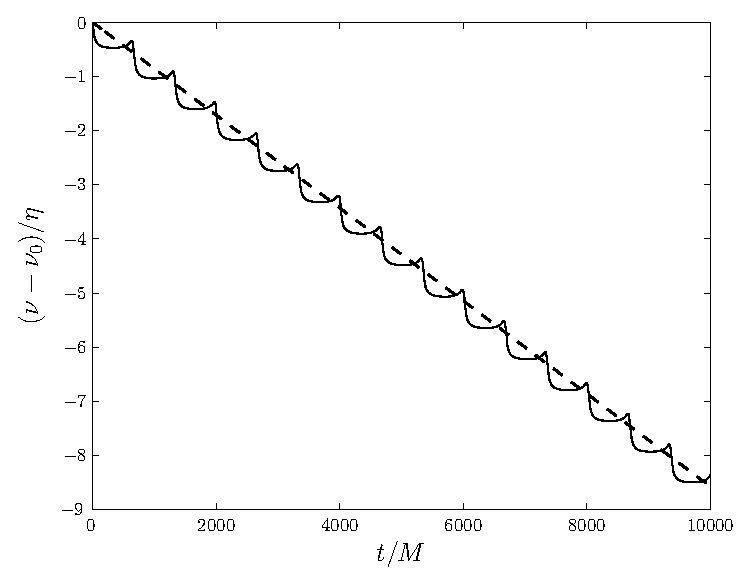
\includegraphics[width=0.46\textwidth]{Fig_ad_vs_inst_wibble}
\caption{\label{fig:wibbles}Evolution of the frequency ratio $\nu$ under both adiabatic (solid line) and instantaneous evolutions. The two coincide at $t = 0$ when $\nu = \nu_0$. The behaviour is general, cf.\ figure 27 of Arnold~\cite{Arnold1988}. In this particular example, $\nu_0 \simeq 0.685$, $\eta = 10^{-6}$ and $a_\ast = 0.9$, the initial orbital parameters are $p = 10$, $e = 0.7$ and $\cos \iota = 0.2$; there are no significant resonances in the plotted span. As a reference for the time-span, the azimuthal orbital period is $T_\phi \simeq 432 M$.}
\end{figure}
However, there shall be a time span when the frequencies are consistently close to being commensurate. During this time the trajectory appears similar to a resonant trajectory, filling only a smaller region of the parameter space. It is this time period that is of interest for transient resonances~\cite{Bosley1992}.

%The Kolmogorov--Arnold--Moser (KAM) theorem states that when an integrable Hamiltonian (i.e., the case for motion in Kerr) is subject to a small perturbation the form of the orbits are preserved albeit slightly deformed~\cite{Arnold1963,Moser1973}. % Chapter II, section 3.3 d)
%When we average the self-force and follow the adiabatic evolution of the trajectory we are exploiting this behaviour. However, the KAM theory only applies for sufficiently incommensurate orbits: close to resonance it does not apply~\cite{Moser1973}. % Chapter V section 1. c)
% In these regions the adiabatic approximation breaks down and we need to follow the instantaneous evolution.

\subsection{Self-force model}

To follow the evolution of the inspiral we must have a means of modelling the self-force. In this work we use the same post-Newtonian approximation as Flanagan and Hinderer~\cite{Flanagan2012}. They use the first-order post-Newtonian terms of the dissipative self-force formulated in Flanagan and Hinderer~\cite{Flanagan2007} and the conservative force formulated in Iyer and Will~\cite{Iyer1993}, and Kidder~\cite{Kidder1995}. Since only the first post-Newtonian terms are used, this prescription can only be of limited validity in strong fields. Both pieces of the self-force are computed assuming that the spin is small: the dissipative piece contains terms to $\order{a_\ast^2}$ and the conservative piece to $\order{a_\ast}$. This is less than ideal for high spins. While this approximate self-force is not perfect, it should serve as a guide for the behaviour of the full self-force.

%For comparison, Flanagan, Hughes and Ruangeri~\cite{Flanagan2012a} use a Teukolsky equation calculation of GW fluxes to account for radiation reaction.

\section{Location of resonances}

The first step in studying the effect of transient resonance is to locate orbital parameters for which the frequencies are commensurate. We can calculate the frequencies and so we are left with the problem of solving $\Omega = n_r \Omega_r - n_\theta \Omega_\theta = 0$ numerically. \Figref{res-plane-2-5-95} shows the semilatus rectum, eccentricity and (cosine of the) inclination angle of the $\nu = 2/5$ resonance surface for a BH of spin $a_\ast = 0.95$. 
\begin{figure}[htbp]
\centering
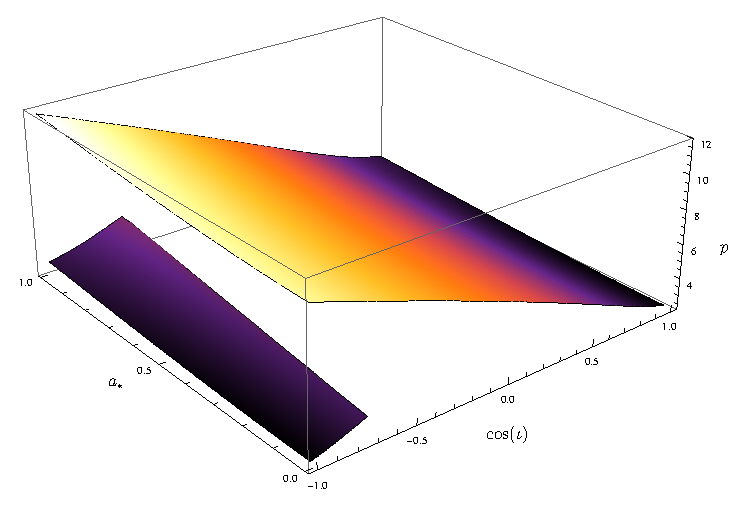
\includegraphics[width=0.46\textwidth]{Fig_res-2-5-95}
\caption{\label{fig:res-plane-2-5-95}Location of the $2/5$ resonance surface for an $a_\ast = 0.95$ BH in terms of orbital semilatus rectum $p$, eccentricity $e$ and inclination $\iota$.}
\end{figure}
The resonances occur at relatively small periapses, corresponding to regions of strong-field gravity.
Similar resonance surfaces can be found for other spin values and for other resonances. When considering the full parameter set of $\{p,e,\iota,a_\ast,\nu\}$ it is apparent that the search for resonances becomes expensive as a consequence of the dimensionality. It is therefore useful to have a guide of where to look. We shall attempt to build a model for the resonance plane.

Brink, Geyer and Hinderer~\cite{Brink2013} provide series expansions for the location of resonances in the limit of equatorial orbits for small spin and eccentricity. We do not follow this approach of trying to find analytic expressions for the resonance surface. The expressions become complicated when venturing away from limiting cases. Instead, we build an approximate phenomenological model and fit this to the resonance plane.%\footnote{A stopped clock is precisely correct twice a day, while a clock that is five minutes slow is never right but will often be close enough. Within this metaphor, our approximation would be a clock that varies between telling the correct time and being fifteen minutes off throughout the day: it is generally going to be good enough to give you a sense of the time but if you have an important event you should check with something better.}
This should be useful for designating the region in which resonance could be expected. To locate them precisely it is necessary to solve $\Omega = 0$ numerically; the approximate model should give a suitable starting point.

The resonant semilatus rectum for any particular spin and resonance ratio can be well approximated as
\begin{equation}
p(e,\iota;a_\ast,\nu) \simeq A\frac{1 + B e + D \cos\iota}{1 + C\exp(e)}.
\end{equation}
The coefficients $\{A,B,C,D\}$ depend upon the spin and the particular resonance; they can be approximated as
\begin{eqnarray} 
A(a_\ast,\nu) & \simeq & a_0\frac{1 + a_1\nu - a_2 \nu^2 - a_3 \nu a_\ast^2}{1 + a_4\nu - (1 + a_4)\nu^2}, \\
B(a_\ast,\nu) & \simeq & b_0(1 - b_1\nu)\exp(-b_2\nu)(1 + b_3 a_\ast), \\
C(a_\ast,\nu) & \simeq & c_0, \\
D(a_\ast,\nu) & \simeq & d_0\left[1 - \exp(a_\ast)\right]\left[1 - d_1\exp(\nu)\right].
\end{eqnarray}
This gives us a total of $12$ parameters for our fit. Whilst this may sound large, if we were fitting an expansion to quadratic order in any combination of $\{e,\iota,a_\ast,\nu\}$ we would have $15$ parameters.\footnote{This does not give as good a fit as our function.} Our optimised parameters are
\begin{equation}
\begin{array}{lll}
a_0 = 5.9854, & a_1 = 3.4116, & a_2 = 0.9253,\\
a_3 = 0.1959, & a_4 = 4.8846, & b_0 = 0.7692,\\
b_1 = 1.4752, & b_2 = 1.4861, & b_3 = -0.5974,\\
c_0 = -0.02332, & d_0 = 0.7968, & d_1 = 0.3115.
\end{array}
\end{equation} 
%These were fitted for resonances with $\nu = 1/7, 1/6, 1/5, 1/4, 2/7, 1/3, 2/5, 3/7, 1/2, 4/7, 3/5, 2/3, 5/7, 3/4, 4/5, 5/6, 6/7, 9/10, 19/20, 49/50, 99/100$, with BH spins of $a_\ast = 0.01, 0.05, 0.1, 0.2, 0.3, 0.4, 0.5, 0.6, 0.7, 0.8, 0.9, 0.93, 0.95, 0.97, 0.99, 0.999$. 
Using this approximation, the maximum error in $p$ for a given $a_\ast$ and $\nu$ is typically $\sim10\%$ and less that $1$ in absolute terms. The relative error in the semilatus rectum is illustrated in \figref{p-error}. 
\begin{figure*}[htp]
\centering
\centerline{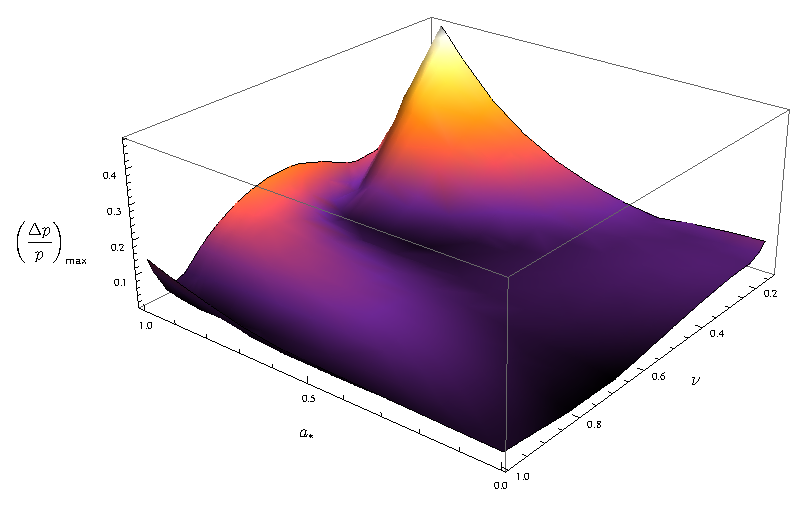
\includegraphics[width=0.47\textwidth]{Fig_fit-error-max}\quad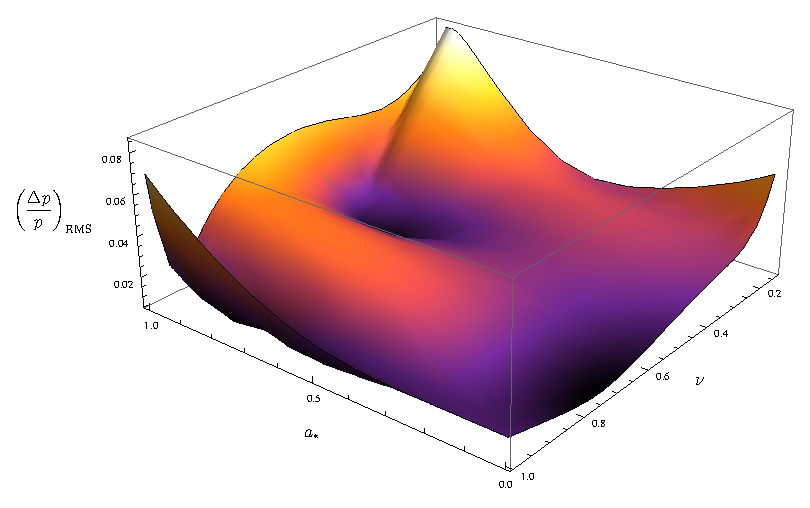
\includegraphics[width=0.47\textwidth]{Fig_fit-error-RMS}}
\caption{\label{fig:p-error}Relative error in the approximate semilatus rectum compared to the accurate numerical result as a function of BH spin $a_\ast$ and resonance ratio $\nu$. The left panel shows the maximum relative error and the right shows the root-mean-square error; in both cases we are marginalising over eccentricity and inclination.}
\end{figure*}
The largest fractional error is $\sim50\%$, this is for $a\rightarrow 1$ and $\nu \rightarrow 0$, and corresponds to small $p$, such that the absolute error is still small. Taking the root-mean-square across $e$ and $\iota$, the fractional error for a given $a_\ast$ and $\nu$ never exceeds $9\%$ and is typically less than $4\%$.

\section{Importance of resonances}

Having determined the location of resonances we may now address their importance. We study the enhancement of the flux of $E$, $L_z$ and $Q$ during resonance and, equivalently, the change in the $p$, $e$ and $\iota$. We also investigate the dephasing in the waveform compared to a purely adiabatic evolution. This is of interest for matched filtering analysis of inspirals.

\subsection{Time-scales}

When analysing resonances it is useful to refer to a number of reference time-scales. We  always use coordinate time $t$, corresponding to what is measured by an observer at infinity, for these. We use the orbital period $T$, the evolution time-scale $\tau\sub{ev}$, the precession time-scale $\tau\sub{pres}$ and the resonance time-scale $\tau\sub{res}$.

The simplest time-scales are the orbital periods $T_r = 2\pi/\Omega_r$, $T_\theta = 2\pi/\Omega_\theta$ and $T_\phi = 2\pi/\Omega_\phi$. These shall be the shortest in our set. We shall use $T$ to denote a time-scale of the same order as the orbital periods.

We define the evolution time-scale as
\begin{equation}
\tau\sub{ev} = \frac{\nu}{\dot{\nu}},
\end{equation}
where an overdot denotes a derivative with respect to $t$. In general, away from resonance, we take $\nu \equiv \Omega_r/\Omega_\theta$. This time-scale sets the period over which there is a significant change in the frequencies. It acts as an inspiral time-scale. It is long in all cases we study, $\tau\sub{ev} \sim \order{T/\eta}$. It is this property which makes extreme-mass-ratio inspirals interesting, as we can follow the waveform for many cycles, accruing high signal-to-noise ratios. This is also what allows us to use the adiabatic prescription, as it means the trajectory moves slowly through different orbital parameters.

We use the precession time-scale
\begin{equation}
\tau\sub{pres}(t) = \frac{2\pi}{|\Omega(t)|},
\label{eq:t-pres}
\end{equation}
with $\Omega(t) = n_r \Omega_r(t) - n_\theta \Omega_\theta(t)$, where the frequencies are calculated instantaneously and the integers are for the resonance of interest. This time-scale becomes infinite exactly on resonance, but decreases as we get further from resonance. It measures the relative precession rate of the radial and poloidal motions and hence gives an indication of how long it takes to fill the entire $\psi$--$\chi$ $2$-torus.

We also use the resonance time-scale
\begin{equation}
\tau\sub{res} = \left[\frac{2\pi}{\left|\langle\dot{\Omega}(0)\rangle_t\right|}\right]^{1/2}.
\label{eq:t-res}
\end{equation}
Here $\dot{\Omega}(0)$ is the rate of change of $\Omega$ at resonance, which we take to be at $t = 0$. The instantaneous $\dot{\Omega}$ depends upon the orbital phase and oscillates about its mean trend over an orbit. We are interested in the averaged behaviour, not the periodic modulations about this, which is why we use the time-average $\langle\dot{\Omega}\rangle_t$. The general trend is that $\Omega$ decreases linearly with time, hence we make the approximation
\begin{equation}
\left|\langle\dot{\Omega}\rangle_t\right| \simeq \left|\frac{\Omega(t)}{t}\right|.
\end{equation}
The resonant time-scale should give an indication of the time over which we expect the effects of the resonance to be felt~\cite{Bosley1992}. Consider the phase of the Mino time Fourier expansion on resonance; neglecting the constant, the resonant Fourier component has form
\begin{equation}
\varphi_{n_r,\,-n_\theta} \simeq \left(n_r\Upsilon_r - n_\theta\Upsilon_\theta\right)\lambda + \left(n_r\dot{\Upsilon_r} - n_\theta\dot{\Upsilon}_\theta\right)\lambda^2 + \ldots
\end{equation}
Typically, the first term is non-zero and this gives the familiar oscillation. On resonance it is zero, leaving the next order term to govern the behaviour~\cite{Flanagan2012}. Only once we have moved far enough away from resonance for the first term to dominate the second do we recapture the non-resonant behaviour. The first term (translating from Mino time to coordinate time) sets $T$, the second sets $\tau\sub{res}$.

Since we have argued that the effect of resonance can be thought of as a consequence of not densely covering the $\psi$--$\chi$ $2$-torus, we might expect that $\tau\sub{pres}$, as well as $\tau\sub{res}$, could be used for setting the resonance duration: the resonance ends once sufficient time has elapsed that the $2$-torus could be filled. This is indeed the case. Let $t\sub{pres}$ be the time taken to fill the torus, then
\begin{eqnarray}
t\sub{pres} & = & \tau\sub{pres}(t\sub{pres}) \\
 & \simeq & \frac{2\pi}{\left|\dot{\Omega}t\sub{pres}\right|}, \nonumber 
\end{eqnarray}
using \eqnref{t-pres} and substituting $\Omega(t\sub{pres}) \simeq \dot{\Omega}t\sub{pres}$. Rearranging and using \eqnref{t-res} gives
\begin{equation}
t\sub{pres} \simeq \tau\sub{res}.
\end{equation}
The two time-scales are equivalent. We shall preferentially use $\tau\sub{res}$ to denote the resonance width. It is shorter than the inspiral time-scale, but longer than an orbital period, $\tau\sub{res} \sim \order{\sqrt{\eta}\tau\sub{ev}} \sim \order{T/\sqrt{\eta}}$~\cite{Flanagan2012,Gair2011a}; it therefore acts as a bridge between the two time-scales~\cite{Hinderer2008}.

Since we shall be considering Fourier decompositions, in anticipation of future results, we shall also define time-scales for the $s$-th resonant frequency harmonic
\begin{eqnarray}
\tau_{\mathrm{pres},\,s} & = & \frac{2\pi}{|s\Omega(t)|};\\
\tau_{\mathrm{res},\,s} & = & \left[\frac{2\pi}{\left|\langle s\dot{\Omega}(0)\rangle_t\right|}\right]^{1/2}.
\end{eqnarray}
These assume that $s$ is a non-zero integer.

\subsection{Resonance enhancement}

\subsection{Dephasing}

\section{Astrophysical implications}


\section{Concluding remarks}

\begin{acknowledgments}
The authors thank Tanja Hinderer, Jeanandrew Brink, Maarten van de Meent and Leor Barack for useful conversations. RHC is supported by STFC; CPLB is supported by STFC and the Cambridge Philosophical Society; PC is supported by a Marie Curie Fellowship, and JRG is supported by the Royal Society.
\end{acknowledgments}

\bibliography{Resonances}

\end{document}
